\documentclass[12pt, a4paper]{article}

% ── Packages ──────────────────────────────────────────────────────────────
\usepackage{geometry}
\geometry{left=2.5cm, right=2.5cm, top=2.8cm, bottom=2.8cm}
\usepackage{booktabs}
\usepackage{longtable}
\usepackage{array}
\usepackage{xcolor}
\usepackage{listings}
\usepackage{hyperref}
\usepackage{amsmath}
\usepackage{amssymb}
\usepackage{enumitem}
\usepackage{fancyhdr}
\usepackage{titlesec}
\usepackage{multirow}
\usepackage{makecell}
\usepackage{tabularx}
\usepackage{tikz}
\usetikzlibrary{shapes.geometric, arrows.meta, positioning, fit, backgrounds}
\usepackage{caption}
\usepackage{subcaption}
\usepackage{microtype}

% ── Header / Footer ───────────────────────────────────────────────────────
\pagestyle{fancy}
\fancyhf{}
\fancyhead[L]{\scriptsize PerturbQA \textemdash\ Gene Perturbation Knowledge Q\&A System}
\fancyhead[R]{\scriptsize Deep Learning \& Life Sciences \textemdash\ AI Agent Project}
\fancyfoot[C]{\thepage}
\renewcommand{\headrulewidth}{0.4pt}
\setlength{\headheight}{14pt}

% ── Colors ────────────────────────────────────────────────────────────────
\definecolor{codegreen}{rgb}{0,0.6,0}
\definecolor{codegray}{rgb}{0.5,0.5,0.5}
\definecolor{codebg}{rgb}{0.97,0.97,0.97}
\definecolor{mainblue}{RGB}{31,73,125}
\definecolor{accentblue}{RGB}{68,114,196}
\definecolor{pigreen}{RGB}{40,120,80}
\definecolor{pilight}{RGB}{220,240,230}

% ── Code listing style ────────────────────────────────────────────────────
\lstset{
  backgroundcolor=\color{codebg},
  basicstyle=\ttfamily\small,
  keywordstyle=\color{mainblue}\bfseries,
  commentstyle=\color{codegreen},
  stringstyle=\color{red!70!black},
  numberstyle=\tiny\color{codegray},
  numbers=left, numbersep=5pt,
  breaklines=true, captionpos=b,
  frame=single, rulecolor=\color{gray!40},
  xleftmargin=1em, framexleftmargin=1em,
}

% ── Hyperlinks ────────────────────────────────────────────────────────────
\hypersetup{colorlinks=true, linkcolor=mainblue, citecolor=accentblue, urlcolor=accentblue}

% ── Section style ─────────────────────────────────────────────────────────
\titleformat{\section}{\large\bfseries\color{mainblue}}{\thesection.}{0.6em}{}[\vspace{-0.4ex}\rule{\linewidth}{0.5pt}]
\titleformat{\subsection}{\normalsize\bfseries\color{accentblue}}{\thesubsection}{0.6em}{}

% ── TikZ node styles ──────────────────────────────────────────────────────
\tikzset{
  agent/.style={rectangle, rounded corners=4pt, draw=mainblue, fill=accentblue!15,
                text width=2.6cm, align=center, minimum height=1.0cm, font=\small\bfseries},
  pibox/.style={rectangle, rounded corners=6pt, draw=pigreen, fill=pilight,
                text width=3.2cm, align=center, minimum height=1.0cm, font=\small\bfseries},
  tool/.style={rectangle, rounded corners=4pt, draw=codegreen!70!black, fill=codegreen!10,
               text width=2.4cm, align=center, minimum height=0.8cm, font=\small},
  store/.style={cylinder, shape border rotate=90, draw=gray!60, fill=gray!10,
                text width=2.4cm, align=center, minimum height=1.0cm, font=\small},
  repl/.style={rectangle, rounded corners=4pt, draw=purple!70, fill=purple!8,
               text width=3.0cm, align=center, minimum height=0.8cm, font=\small},
  arrow/.style={-{Stealth[length=6pt]}, thick, color=gray!70},
  dasharrow/.style={-{Stealth[length=6pt]}, dashed, thick, color=accentblue!70},
  piarrow/.style={-{Stealth[length=6pt]}, thick, color=pigreen!80},
}

% ─────────────────────────────────────────────────────────────────────────
\begin{document}

% ══ Title page ════════════════════════════════════════════════════════════
\begin{titlepage}
  \centering
  \vspace*{2cm}
  {\LARGE\bfseries\color{mainblue} Deep Learning \& Life Sciences}\\[0.6em]
  {\large AI Agent Course Project Report}\\[2cm]

  {\Huge\bfseries PerturbQA}\\[0.5em]
  {\large\color{accentblue}
    Gene Perturbation Knowledge Q\&A System\\[0.3em]
    via Pi Extension, Agentic RAG, and Iterative Tool-Calling}\\[2.5cm]

  \begin{tabular}{rl}
    \textbf{Research Topic}      & \texttt{gene-perturbation}\\[0.4em]
    \textbf{Stack}               & TypeScript / Node.js / \texttt{@earendil-works/pi-ai}\\[0.4em]
    \textbf{Infrastructure}      & Pi TUI extension\\[0.4em]
    \textbf{Knowledge Sets}      & \textbf{51} (from 47 curated academic papers, 2012--2026)\\[0.4em]
    \textbf{Vector Store}        & 82 indexed chunks (cosine similarity + BM25 bigram)\\[0.4em]
    \textbf{Benchmark Questions} & 22 across 5 types, 3 difficulty levels\\[0.4em]
    \textbf{Optional Modules}    & Skills Lv.2 + Memory Lv.1 + Orchestration Lv.1\\
                                 & (difficulty sum $= 4$, meets requirement $\ge 4$)\\[0.4em]
    \textbf{Best Benchmark}      & \textbf{54.5\% pass rate, 62.0/100 avg}\\
                                 & (Claude Sonnet 4.6, pi-agent mode)\\
  \end{tabular}

  \vfill
  {\large June 2026}
\end{titlepage}

% ══ Table of contents ═════════════════════════════════════════════════════
\tableofcontents
\newpage

% ══════════════════════════════════════════════════════════════════════════
\section{Project Overview}
% ══════════════════════════════════════════════════════════════════════════

PerturbQA is an intelligent Q\&A system for the \textbf{gene perturbation} domain.
It is implemented as a \textbf{pi extension} --- a plugin that runs inside the Pi TUI
(terminal user interface) rather than as a standalone REPL. This design inherits pi's
streaming output, markdown rendering, session persistence, and model management for free,
while injecting domain-specific tools and a structured system prompt.

The system supports any model provider authenticated through pi's credential store
(\texttt{\textasciitilde/.perturbqa/agent/auth.json}): Claude Sonnet/Opus, GPT-4o/5,
Gemini, and any locally hosted model. All LLM calls are routed through
\texttt{@earendil-works/pi-ai}'s \texttt{completeSimple()} / \texttt{complete()},
which handles OAuth token refresh, rate-limit retry, and provider normalisation.

\subsection{Module Selection and Scoring}

\begin{table}[h]
\centering
\caption{Selected modules and expected scores}
\begin{tabularx}{\textwidth}{lXccc}
\toprule
\textbf{Module} & \textbf{Selection} & \textbf{Max} & \textbf{Diff.} & \textbf{Weight} \\
\midrule
Knowledge Assets     & \textbf{51} knowledge sets ($\ge20$)  & 35  & ---   & independent \\
Evaluation Benchmark & 22 questions ($\ge20$)                & 35  & ---   & independent \\
\midrule
Q\&A --- Skills      & Domain MCP Tools (Lv.2)               & 100 & 2     & $2/4 = 0.50$ \\
Q\&A --- Memory      & Agentic RAG (Lv.1)                    & 100 & 1     & $1/4 = 0.25$ \\
Q\&A --- Orchestration & Pi-Agent + 4-Agent Pipeline (Lv.1) & 100 & 1     & $1/4 = 0.25$ \\
\midrule
\multicolumn{2}{l}{Q\&A Project Final Score} & 30 & \multicolumn{2}{c}{weighted avg $\times\ 0.3$} \\
\bottomrule
\end{tabularx}
\end{table}

Difficulty sum $= 2+1+1 = 4$, satisfying the course requirement ($\ge 4$).

\subsection{System Architecture}

PerturbQA runs as a subprocess inside pi's TUI engine:

\begin{figure}[ht]
\centering
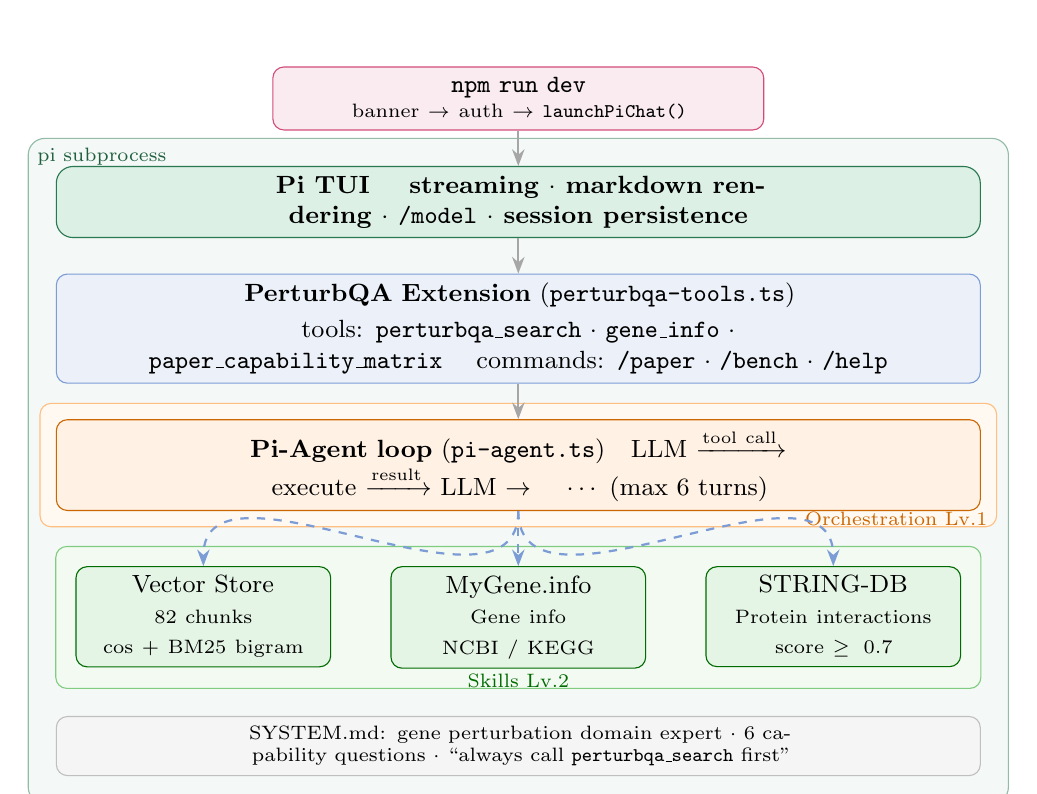
\begin{tikzpicture}[node distance=0.55cm]

  % ── Entry point ──────────────────────────────────────────────────────
  \node[repl, text width=6cm, minimum height=0.8cm] (entry)
    {\texttt{npm run dev}\\[-2pt]
     {\scriptsize banner $\rightarrow$ auth $\rightarrow$ \texttt{launchPiChat()}}};

  \draw[arrow] (entry.south) -- ++(0,-0.45);

  % ── Pi TUI ───────────────────────────────────────────────────────────
  \node[pibox, text width=11.5cm, minimum height=0.85cm,
        below=0.45cm of entry] (pitui)
    {\textbf{Pi TUI} \quad {\small streaming $\cdot$ markdown rendering $\cdot$ \texttt{/model} $\cdot$ session persistence}};

  \draw[arrow] (pitui.south) -- ++(0,-0.45);

  % ── Extension ────────────────────────────────────────────────────────
  \node[rectangle, draw=accentblue!70, fill=accentblue!10, rounded corners=4pt,
        text width=11.5cm, minimum height=1.1cm, align=center, font=\small,
        below=0.45cm of pitui] (ext)
    {\textbf{PerturbQA Extension} (\texttt{perturbqa-tools.ts})\\[2pt]
     tools: \texttt{perturbqa\_search} $\cdot$ \texttt{gene\_info} $\cdot$ \texttt{paper\_capability\_matrix}
     \quad commands: \texttt{/paper} $\cdot$ \texttt{/bench} $\cdot$ \texttt{/help}};

  \draw[arrow] (ext.south) -- ++(0,-0.45);

  % ── Pi-Agent loop ─────────────────────────────────────────────────────
  \node[rectangle, draw=orange!80!black, fill=orange!10, rounded corners=4pt,
        text width=11.5cm, minimum height=0.85cm, align=center, font=\small,
        below=0.45cm of ext] (agent)
    {\textbf{Pi-Agent loop} (\texttt{pi-agent.ts})\quad
     LLM $\xrightarrow{\text{tool call}}$ execute $\xrightarrow{\text{result}}$ LLM $\rightarrow \cdots$ (max 6 turns)};

  % ── Tool nodes ────────────────────────────────────────────────────────
  \node[tool, text width=3.0cm, minimum height=1.1cm,
        below=0.7cm of agent, xshift=-4.0cm] (t1)
    {Vector Store\\{\scriptsize 82 chunks}\\{\scriptsize cos $+$ BM25 bigram}};

  \node[tool, text width=3.0cm, minimum height=1.1cm,
        below=0.7cm of agent] (t2)
    {MyGene.info\\{\scriptsize Gene info}\\{\scriptsize NCBI / KEGG}};

  \node[tool, text width=3.0cm, minimum height=1.1cm,
        below=0.7cm of agent, xshift=4.0cm] (t3)
    {STRING-DB\\{\scriptsize Protein interactions}\\{\scriptsize score $\ge 0.7$}};

  \draw[dasharrow] (agent.south) to[out=270,in=90] (t1.north);
  \draw[dasharrow] (agent.south) -- (t2.north);
  \draw[dasharrow] (agent.south) to[out=270,in=90] (t3.north);

  % ── System prompt ─────────────────────────────────────────────────────
  \node[rectangle, draw=gray!50, fill=gray!8, rounded corners=4pt,
        text width=11.5cm, minimum height=0.75cm, align=center, font=\scriptsize,
        below=0.6cm of t2] (sysp)
    {SYSTEM.md: gene perturbation domain expert $\cdot$
     6 capability questions $\cdot$
     ``always call \texttt{perturbqa\_search} first''};

  % ── Background boxes ──────────────────────────────────────────────────
  \begin{pgfonlayer}{background}
    \node[rectangle, rounded corners=6pt, draw=pigreen!50, fill=pigreen!5,
          fit=(pitui)(ext)(agent)(t1)(t2)(t3)(sysp),
          inner sep=0.35cm] (subproc) {};
    \node[anchor=north west, font=\scriptsize\color{pigreen!80!black}]
          at (subproc.north west) {pi subprocess};

    \node[rectangle, rounded corners=4pt, draw=codegreen!50, fill=codegreen!5,
          fit=(t1)(t2)(t3), inner sep=0.25cm] (skillbox) {};
    \node[anchor=south, font=\scriptsize\color{codegreen!70!black},
          yshift=-3pt] at (skillbox.south) {Skills Lv.2};

    \node[rectangle, rounded corners=4pt, draw=orange!50, fill=orange!5,
          fit=(agent), inner sep=0.2cm] (orchbox) {};
    \node[anchor=south east, font=\scriptsize\color{orange!80!black},
          yshift=-3pt] at (orchbox.south east) {Orchestration Lv.1};
  \end{pgfonlayer}

\end{tikzpicture}
\caption{PerturbQA system architecture (pi extension approach)}
\end{figure}

% ══════════════════════════════════════════════════════════════════════════
\section{Knowledge Assets (35 pts)}
% ══════════════════════════════════════════════════════════════════════════

\subsection{Collection Overview}

The knowledge base contains \textbf{51 knowledge sets} sourced from \textbf{47 peer-reviewed
papers} spanning 2012--2026.  Each knowledge set has three standardised files:
\begin{itemize}[nosep]
  \item \texttt{content/<slug>.md} --- 800--2000-word structured summary, including a
        \textbf{Capability Summary} table for all prediction-model entries (see \S\ref{sec:extra});
  \item \texttt{keywords.json} --- topic tag and keyword list;
  \item \texttt{source.json} --- full bibliographic metadata (DOI, authors, journal, year).
\end{itemize}
All directory names use kebab-case as required.
The vector store indexes \textbf{82 chunks} from the 51 knowledge sets
(Capability Summary sections are embedded as separate retrievable chunks).

\subsection{Original 24 Knowledge Sets}

\begin{longtable}{@{}p{0.5cm}p{5.4cm}p{3.2cm}p{3.6cm}@{}}
\caption{Original 24 knowledge sets (first batch)} \label{tab:kb1} \\
\toprule
\textbf{\#} & \textbf{Title} & \textbf{Year / Venue} & \textbf{Category} \\
\midrule
\endfirsthead
\multicolumn{4}{l}{\small(continued)} \\
\toprule
\textbf{\#} & \textbf{Title} & \textbf{Year / Venue} & \textbf{Category} \\
\midrule
\endhead
\bottomrule
\endfoot
1  & CRISPR-Cas9 Mechanism of DNA Cleavage        & 2012, \textit{Science}              & Core mechanism \\
2  & CRISPR Pooled Screens: Design and Analysis    & 2014, \textit{Science}              & Experimental method \\
3  & Perturb-seq: CRISPR with scRNA-seq            & 2016, \textit{Cell}                 & Experimental method \\
4  & Gene Regulatory Network Inference             & 2019, \textit{Science}              & Regulatory network \\
5  & GEARS: GNN for Perturbation Prediction        & 2023, \textit{Nature Biotechnology} & Prediction (GNN) \\
6  & CPA Compositional Perturbation Autoencoder    & 2023, \textit{Mol. Systems Biol.}   & Prediction (VAE) \\
7  & CRADLE-VAE Artifact Disentanglement           & 2024, \textit{AAAI 2025}            & Prediction (VAE) \\
8  & scGPT Foundation Model                        & 2024, \textit{Nature Methods}       & Foundation model \\
9  & Scouter LLM-Based Perturbation Prediction     & 2024, \textit{bioRxiv}              & Prediction (LLM) \\
10 & TranSiGen Chemical Perturbation VAE           & 2024, \textit{Nature Communications}& Prediction (drug) \\
11 & AUPRC Metric for DEG Evaluation               & 2025, \textit{Briefings Bioinform.} & Evaluation \\
12 & CellFlow Flow Matching for Single-Cell         & 2025, \textit{bioRxiv}              & Prediction (flow) \\
13 & GPO-VAE GRN-Aligned Perturbation Modeling     & 2025, \textit{arXiv}                & Prediction (VAE) \\
14 & Linear Baseline Benchmark                     & 2025, \textit{Nature Methods}       & Evaluation \\
15 & Miller et al.\ Dynamic Range Fraction         & 2025, \textit{bioRxiv}              & Evaluation \\
16 & Systema Evaluation Framework                  & 2025, \textit{Nature Biotechnology} & Evaluation \\
17 & TxPert OOD Transcriptomic Prediction          & 2025, \textit{Nature Biotechnology} & Prediction (GNN) \\
18 & Unlasting Dual Conditional Diffusion          & 2025, \textit{arXiv}                & Prediction (diffusion) \\
19 & AdaPert Adaptive Perturbation Context         & 2026, \textit{arXiv}                & Prediction (GNN) \\
20 & GGE Standardised Evaluation Framework         & 2026, \textit{ICLR 2026 Gen$^2$}   & Evaluation \\
21 & PerturbDiff Functional Diffusion              & 2026, \textit{arXiv}                & Prediction (diffusion) \\
22 & PerturbedVAE Causal Representation            & 2026, \textit{ICML 2026}            & Prediction (VAE) \\
23 & PerturbGraph GNN with Biological Priors       & 2026, \textit{bioRxiv}              & Prediction (GNN) \\
24 & scBIG Module-Inductive Perturbation           & 2026, \textit{arXiv}                & Prediction (GNN) \\
\end{longtable}

\subsection{Additional 27 Knowledge Sets (Second Batch)}

\begin{longtable}{@{}p{0.5cm}p{5.4cm}p{3.2cm}p{3.6cm}@{}}
\caption{New 27 knowledge sets (second batch)} \label{tab:kb2} \\
\toprule
\textbf{\#} & \textbf{Title} & \textbf{Year / Venue} & \textbf{Category} \\
\midrule
\endfirsthead
\multicolumn{4}{l}{\small(continued)} \\
\toprule
\textbf{\#} & \textbf{Title} & \textbf{Year / Venue} & \textbf{Category} \\
\midrule
\endhead
\bottomrule
\endfoot
25 & CellFM: 100M Human Cell Foundation Model     & 2025, \textit{Nature Communications} & Foundation model \\
26 & EpiAgent: Single-Cell Epigenomics Foundation  & 2025, \textit{Nature Methods}        & Foundation model \\
27 & GeneCompass: Cross-Species Foundation Model   & 2024, \textit{Cell Research}         & Foundation model \\
28 & RegFormer: GRN-Hierarchy Mamba Foundation     & 2026, \textit{Nature Communications} & Foundation model \\
29 & scFoundation: 100M Asymmetric Transformer     & 2024, \textit{Nature Methods}        & Foundation model \\
30 & scLong: 1B-Parameter Long-Context Model       & 2026, \textit{Nature Communications} & Foundation model \\
31 & Geneformer: Scaling Laws and Quantization     & 2026, \textit{Nat.\ Computational Sci.} & Foundation model \\
32 & GPerturb: Gaussian Process for Perturbation   & 2025, \textit{Nature Communications} & Prediction (GP) \\
33 & Squidiff: Diffusion for Perturbation Response & 2025, \textit{Nature Methods}        & Prediction (diffusion) \\
34 & Departures: Neural Schr\"{o}dinger Bridge     & 2026, \textit{AAAI 2026}             & Prediction (bridge) \\
35 & PDGrapher: Causal GNN for Therapeutics        & 2025, \textit{Nat.\ Biomedical Eng.} & Prediction (causal) \\
36 & STAMP: Subtask Decomposition for Perturbation & 2024, \textit{Nat.\ Computational Sci.} & Prediction (GNN) \\
37 & XPert: Dual-Branch Drug Perturbation          & 2026, \textit{Nat.\ Machine Intelligence} & Prediction (drug) \\
38 & PrePR-CT: Graph Drug Response                 & 2026, \textit{Nat.\ Machine Intelligence} & Prediction (drug) \\
39 & PRnet: Generative Chemical Perturbation Model & 2024, \textit{Nature Communications} & Prediction (drug) \\
40 & LPM: Large Perturbation Model                 & 2025, \textit{Nat.\ Computational Sci.} & Prediction (foundation) \\
41 & Biolord: Single-Cell Multi-Omic Disentanglement & 2024, \textit{Nature Biotechnology} & Prediction (disentanglement) \\
42 & scVAEDer: VAE $+$ Diffusion for Single-Cell   & 2025, \textit{Genome Biology}        & Prediction (VAE+diff.) \\
43 & MorphDiff: Transcriptome-Guided Morphology    & 2025, \textit{Nature Communications} & Prediction (diffusion) \\
44 & Pertpy: End-to-End Perturbation Framework     & 2025, \textit{Nature Methods}        & Analysis tool \\
45 & scDist: Mixed-Effects Perturbed Cell Types    & 2024, \textit{Nature Communications} & Analysis tool \\
46 & scDNS: Network Divergence Analysis            & 2026, \textit{Nature Communications} & Analysis tool \\
47 & River: Interpretable DL for Spatial           & 2025, \textit{Nature Communications} & Analysis tool \\
48 & CPJUMP1: Image-Based Perturbation Benchmark   & 2024, \textit{Nature Methods}        & Benchmark \\
49 & 27-Method Generalisation Benchmark            & 2025, \textit{Nature Methods}        & Benchmark \\
50 & Perturbation-Response Score (PS)              & 2025, \textit{Nature Cell Biology}   & Evaluation \\
51 & Mixscale: Scalable Perturb-seq Pathways       & 2025, \textit{Nature Cell Biology}   & Experimental method \\
\end{longtable}

\subsection{Coverage Analysis}

\begin{table}[ht]
\centering
\caption{Knowledge set distribution by category (51 total)}
\begin{tabular}{lcc}
\toprule
\textbf{Category} & \textbf{Count} & \textbf{\%} \\
\midrule
Prediction models --- GNN / graph / causal & 9  & 17.6\% \\
Prediction models --- VAE / generative     & 6  & 11.8\% \\
Prediction models --- diffusion \& flow    & 6  & 11.8\% \\
Prediction models --- drug response        & 5  &  9.8\% \\
Foundation models                          & 8  & 15.7\% \\
Evaluation frameworks \& benchmarks        & 9  & 17.6\% \\
Analysis tools                             & 4  &  7.8\% \\
Core mechanism \& experimental methods     & 4  &  7.8\% \\
\midrule
\textbf{Total} & \textbf{51} & \textbf{100\%} \\
\bottomrule
\end{tabular}
\end{table}

% ══════════════════════════════════════════════════════════════════════════
\section{Evaluation Benchmark (35 pts)}
% ══════════════════════════════════════════════════════════════════════════

\subsection{Construction Method}

The benchmark contains \textbf{22 questions} stored in \texttt{benchmark/questions.json}.
Each entry follows the schema:

\begin{lstlisting}[caption={Benchmark question schema (gp-004)}]
{
  "id": "gp-004",
  "question": "What is GEARS and how does it predict transcriptional
               responses to genetic perturbations?",
  "answer": "GEARS (Graph-Enhanced Activation for RNA-Seq Simulation)...",
  "source": {
    "type": "paper",
    "doi": "10.1038/s41587-023-01905-6",
    "title": "Predicting transcriptional outcomes of novel multigene
              perturbations with GEARS"
  },
  "topic": "gene-perturbation",
  "difficulty": "hard",
  "type": "mechanistic"
}
\end{lstlisting}

\subsection{Distribution Statistics}

\begin{table}[ht]
\centering
\caption{Benchmark distribution (22 questions total)}
\begin{subtable}[t]{0.45\textwidth}
\centering
\caption{By question type}
\begin{tabular}{lcc}
\toprule
\textbf{Type} & \textbf{Count} & \textbf{\%} \\
\midrule
comparative & 6 & 27.3\% \\
analytical  & 5 & 22.7\% \\
mechanistic & 4 & 18.2\% \\
procedural  & 4 & 18.2\% \\
factual     & 3 & 13.6\% \\
\midrule
\textbf{Total} & \textbf{22} & \textbf{100\%} \\
\bottomrule
\end{tabular}
\end{subtable}
\hfill
\begin{subtable}[t]{0.45\textwidth}
\centering
\caption{By difficulty}
\begin{tabular}{lcc}
\toprule
\textbf{Difficulty} & \textbf{Count} & \textbf{\%} \\
\midrule
hard   & 8  & 36.4\% \\
medium & 11 & 50.0\% \\
easy   &  3 & 13.6\% \\
\midrule
\textbf{Total} & \textbf{22} & \textbf{100\%} \\
\bottomrule
\end{tabular}
\end{subtable}
\end{table}

\subsection{Representative Questions}

\begin{table}[ht]
\centering
\caption{Sample questions across types and difficulties}
\begin{tabularx}{\textwidth}{lllX}
\toprule
\textbf{ID} & \textbf{Type} & \textbf{Diff.} & \textbf{Question} \\
\midrule
gp-001 & mechanistic & medium & What is the mechanism by which CRISPR-Cas9 creates double-strand breaks? \\
gp-004 & mechanistic & hard   & What is GEARS and how does it predict transcriptional responses? \\
gp-009 & comparative & medium & What is CROP-seq and how does it differ from Perturb-seq? \\
gp-012 & analytical  & medium & What is synthetic lethality and why is it therapeutically relevant? \\
gp-013 & comparative & hard   & How does base editing differ from prime editing? \\
gp-016 & mechanistic & hard   & How does CPA model combinatorial perturbation effects? \\
gp-020 & mechanistic & hard   & How does scGPT use perturbation data for transfer learning? \\
\bottomrule
\end{tabularx}
\end{table}

\noindent The complete question list with reference answer summaries is in Appendix~\ref{app:questions}.

% ══════════════════════════════════════════════════════════════════════════
% APPENDIX MARKER (full question list and case studies moved to end)
% ══════════════════════════════════════════════════════════════════════════

\subsection{Benchmark Execution}

The benchmark is run via the \texttt{/bench} slash command in the pi TUI, or directly:

\begin{lstlisting}[language=bash, caption={Running the benchmark}]
# In pi TUI (after npm run dev):
/bench              # run all 22 questions
/bench gp-001 gp-002 gp-005   # run specific questions by ID

# Direct (bypasses pi TUI, uses pi-agent mode):
node_modules/.bin/tsx src/evaluation/runner.ts
node_modules/.bin/tsx src/evaluation/runner.ts gp-001 gp-005
\end{lstlisting}

\noindent Each question goes through the pi-agent loop (Figure~\ref{fig:piagent}): the LLM
iteratively calls \texttt{perturbqa\_search()} until it has sufficient context, then writes
the final answer. The result is scored by an LLM judge (autoScore) against the reference answer.

\begin{figure}[ht]
\centering
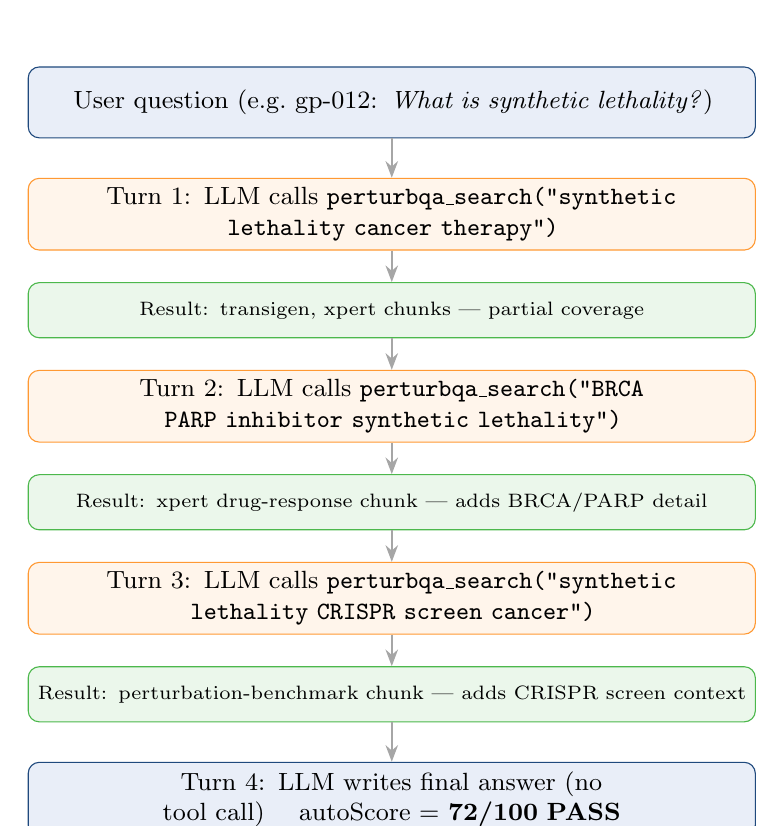
\begin{tikzpicture}[node distance=0.5cm]
  \node[rectangle, draw=mainblue, fill=accentblue!12, rounded corners,
        text width=9cm, minimum height=0.9cm, align=center, font=\small]
    (q) {User question (e.g.\ gp-012: \textit{What is synthetic lethality?})};

  \node[rectangle, draw=orange!80, fill=orange!8, rounded corners,
        text width=9cm, minimum height=0.8cm, align=center, font=\small,
        below=0.5cm of q]
    (t1) {Turn 1: LLM calls \texttt{perturbqa\_search("synthetic lethality cancer therapy")}};

  \node[rectangle, draw=codegreen!70, fill=codegreen!8, rounded corners,
        text width=9cm, minimum height=0.7cm, align=center, font=\scriptsize,
        below=0.4cm of t1]
    (r1) {Result: transigen, xpert chunks — partial coverage};

  \node[rectangle, draw=orange!80, fill=orange!8, rounded corners,
        text width=9cm, minimum height=0.8cm, align=center, font=\small,
        below=0.4cm of r1]
    (t2) {Turn 2: LLM calls \texttt{perturbqa\_search("BRCA PARP inhibitor synthetic lethality")}};

  \node[rectangle, draw=codegreen!70, fill=codegreen!8, rounded corners,
        text width=9cm, minimum height=0.7cm, align=center, font=\scriptsize,
        below=0.4cm of t2]
    (r2) {Result: xpert drug-response chunk — adds BRCA/PARP detail};

  \node[rectangle, draw=orange!80, fill=orange!8, rounded corners,
        text width=9cm, minimum height=0.8cm, align=center, font=\small,
        below=0.4cm of r2]
    (t3) {Turn 3: LLM calls \texttt{perturbqa\_search("synthetic lethality CRISPR screen cancer")}};

  \node[rectangle, draw=codegreen!70, fill=codegreen!8, rounded corners,
        text width=9cm, minimum height=0.7cm, align=center, font=\scriptsize,
        below=0.4cm of t3]
    (r3) {Result: perturbation-benchmark chunk — adds CRISPR screen context};

  \node[rectangle, draw=mainblue, fill=accentblue!12, rounded corners,
        text width=9cm, minimum height=0.9cm, align=center, font=\small,
        below=0.5cm of r3]
    (ans) {Turn 4: LLM writes final answer (no tool call) \quad autoScore = \textbf{72/100 PASS}};

  \draw[arrow] (q) -- (t1);
  \draw[arrow] (t1) -- (r1);
  \draw[arrow] (r1) -- (t2);
  \draw[arrow] (t2) -- (r2);
  \draw[arrow] (r2) -- (t3);
  \draw[arrow] (t3) -- (r3);
  \draw[arrow] (r3) -- (ans);
\end{tikzpicture}
\caption{Pi-agent turn-by-turn trace for gp-012 (synthetic lethality, 3 searches, score 72)}
\label{fig:piagent}
\end{figure}

% ══════════════════════════════════════════════════════════════════════════
\section{Knowledge Q\&A Project (30 pts)}
% ══════════════════════════════════════════════════════════════════════════

\subsection{Skills Module: Domain MCP Tools (Lv.2, difficulty 2)}

\subsubsection{Implementation}

Three domain tool interfaces are implemented and exposed both as MCP tools
(via \texttt{src/mcp/server.ts}) and as pi extension tools
(via \texttt{perturbqa-tools.ts}):

\begin{table}[ht]
\centering
\caption{Domain tool interfaces}
\begin{tabularx}{\textwidth}{llX}
\toprule
\textbf{Tool} & \textbf{Data source} & \textbf{Description} \\
\midrule
\texttt{gene\_info}              & MyGene.info REST API  & Gene symbol, name, species, Entrez ID, summary \\
\texttt{protein\_interactions}   & STRING-DB API v11.5   & Top-10 interacting proteins (combined score $\ge 0.7$) \\
\texttt{paper\_capability\_matrix} & VectorStore + LLM   & 6-question capability evaluation for a paper slug \\
\bottomrule
\end{tabularx}
\end{table}

Tools are registered as pi extension tools so the LLM in the pi TUI can call them
during any conversation with no special syntax:

\begin{lstlisting}[caption={Example: pi TUI automatically calls gene\_info}]
User: What are the interaction partners of BRCA1?

[LLM calls: protein_interactions("BRCA1")]
[Tool result: {gene: "BRCA1", interactions: [{partner: "BARD1", score: 0.999}, ...]}]

BRCA1's top interaction partners include BARD1 (score 0.999), RAD51 (0.997),
BRIP1 (0.983)...
\end{lstlisting}

\subsubsection{Grading Alignment}

\begin{table}[ht]
\centering
\caption{Lv.2 Skills module grading alignment}
\begin{tabular}{lcp{7cm}}
\toprule
\textbf{Criterion} & \textbf{Max} & \textbf{Evidence} \\
\midrule
Project selection    & 15 & MyGene.info (NCBI official) + STRING-DB ($>$6.7B interactions) \\
Function coverage    & 25 & 3 independent tool interfaces ($\ge3$ for full marks) \\
Interface correctness & 25 & HTTP requests validated; structured JSON responses \\
Documentation        & 20 & README + REPORT cover tool description, config, examples \\
Runnability          & 15 & Tools invocable from pi TUI; no runtime errors \\
\bottomrule
\end{tabular}
\end{table}

% ─────────────────────────────────────────────────────────────────────────
\subsection{Memory Module: Agentic RAG (Lv.1, difficulty 1)}

\subsubsection{Design}

The system implements two retrieval paths:

\paragraph{Legacy Agentic RAG} (\texttt{src/rag/agentic-rag.ts}) --- used by the
\texttt{QAOrchestrator} pipeline. An LLM autonomously decides retrieval strategy:

\begin{enumerate}[nosep]
  \item \textbf{Query analysis}: outputs strategy (\texttt{semantic}/\texttt{keyword}/\texttt{hybrid}/\texttt{none}) and query variants;
  \item \textbf{Round 1 retrieval}: execute chosen strategy;
  \item \textbf{Sufficiency check}: LLM reads top-3 snippets, decides if enough;
  \item \textbf{Query refinement + rounds 2--3} if insufficient, with cross-round deduplication.
\end{enumerate}

\medskip\noindent\textbf{Pi-agent inline search} (\texttt{pi-agent.ts}): the LLM
directly calls \texttt{perturbqa\_search()} as a tool, choosing query text and how
many times to search. Both paths share the same hybrid retrieval engine:

\begin{itemize}[nosep]
  \item \textbf{Semantic}: cosine similarity on \texttt{all-MiniLM-L6-v2} embeddings (384-dim, via Xenova);
  \item \textbf{BM25 bigram}: unigram + bigram extraction with $2\times$ weight for phrase matches
        and $3\times$ title bonus --- specifically improves recall for compound terms such as
        ``synthetic lethality'', ``base editing'', ``prime editing'';
  \item \textbf{Hybrid merge}: union by document ID, sort by max score, top-5 returned.
\end{itemize}

\subsubsection{Embedding Model Ablation}

During development we evaluated two embedding models:

\begin{table}[ht]
\centering
\caption{Embedding model comparison on this corpus}
\begin{tabular}{lccp{4.5cm}}
\toprule
\textbf{Model} & \textbf{Dims} & \textbf{Score range} & \textbf{Result} \\
\midrule
\texttt{all-MiniLM-L6-v2} & 384 & 0.20--0.80 & Clear discrimination; correct top-1 \\
\texttt{bge-large-en-v1.5} & 1024 & 0.65--0.85 & Near-zero variance; wrong top-1 for 2/4 test queries \\
\bottomrule
\end{tabular}
\end{table}

BGE-Large (335M parameters, trained for dense retrieval) failed on this small
specialised corpus: all 82 documents fall into a narrow semantic neighbourhood, causing
cosine similarity scores to cluster with $<0.005$ separation between relevant and
irrelevant documents.  We reverted to MiniLM.

\subsubsection{Grading Alignment}

\begin{table}[ht]
\centering
\caption{Lv.1 Agentic RAG module grading alignment}
\begin{tabular}{lcp{7cm}}
\toprule
\textbf{Criterion} & \textbf{Max} & \textbf{Evidence} \\
\midrule
Question set size ($\ge10$) & 10 & 22 benchmark questions \\
Question diversity          & 10 & Factual, mechanistic, comparative, analytical, procedural \\
Retrieval decision ability  & 35 & LLM autonomously selects strategy + query text \\
Retrieval execution         & 15 & Hybrid search with cross-round deduplication \\
Answer quality              & 10 & Answers grounded in retrieved context \\
Runnability                 & 10 & Runs error-free; timeout protection (90s per call) \\
Decision display            &  5 & Per-round trace visible in benchmark output \\
\bottomrule
\end{tabular}
\end{table}

% ─────────────────────────────────────────────────────────────────────────
\subsection{Orchestration Module: Pi-Agent + 4-Agent Pipeline (Lv.1, difficulty 1)}

\subsubsection{Architecture A: Static 4-Agent Pipeline (QAOrchestrator)}

\texttt{QAOrchestrator} (\texttt{src/agents/orchestrator.ts}) coordinates four
independent agents in a fixed serial pipeline, each making one LLM call:

\begin{table}[ht]
\centering
\caption{Four-agent roles, inputs, and outputs}
\begin{tabularx}{\textwidth}{llXX}
\toprule
\textbf{Agent} & \textbf{File} & \textbf{Input} & \textbf{Output} \\
\midrule
\textbf{PlannerAgent}   & \texttt{planner.ts}   & User question & Question type, complexity, keywords, strategy (JSON) \\
\textbf{RetrieverAgent} & \texttt{retriever.ts} & Plan + store & Agentic RAG result (up to 3 rounds), source list \\
\textbf{GeneratorAgent} & \texttt{generator.ts} & Question + context & Grounded, cited answer draft \\
\textbf{ValidatorAgent} & \texttt{validator.ts} & Q + draft + context & Score 0--100, checks, improved answer (JSON) \\
\bottomrule
\end{tabularx}
\end{table}

\subsubsection{Architecture B: Pi-Agent (Iterative Tool-Calling)}

\texttt{runWithPiAgent()} (\texttt{src/agents/pi-agent.ts}) replaces the fixed pipeline
with an LLM-driven iterative loop using \texttt{complete()} from \texttt{@earendil-works/pi-ai}:

\begin{lstlisting}[language=bash, caption={Pi-agent loop pseudocode}]
messages = [{role: "user", content: question}]
for turn in 0..MAX_TURNS:
    response = complete(model, {systemPrompt, messages, tools:[search]})
    messages.append(response)
    if response.stopReason != "toolUse":
        return extractText(response)  # final answer
    for toolCall in response.toolCalls:
        result = executeSearch(toolCall.arguments.query, store)
        messages.append({role:"toolResult", content: result})
\end{lstlisting}

Key parameters: \texttt{MAX\_TURNS = 6}, \texttt{LLM\_TIMEOUT\_MS = 90000},
\texttt{maxTokens = 2048} per call.

The system prompt (\texttt{SYSTEM.md}) instructs the LLM to call \texttt{perturbqa\_search}
at least once, refine if insufficient, and ground every claim in retrieved context.

\subsubsection{Pipeline Comparison}

\begin{table}[ht]
\centering
\caption{Architectural comparison: QAOrchestrator vs pi-agent}
\begin{tabular}{lll}
\toprule
\textbf{Property} & \textbf{QAOrchestrator} & \textbf{Pi-Agent} \\
\midrule
Search decisions  & Fixed (Planner decides once) & LLM iterates dynamically \\
Avg searches/question & 1--3 rounds & 2--4 tool calls \\
JSON parsing      & Manual regex fallback & Native pi-ai tool schema \\
Context window    & Per-agent slice & Full message history \\
Validation        & Separate ValidatorAgent & autoScore judge (external) \\
Benchmark pass rate & 40.9\% & \textbf{54.5\%} \\
Avg score         & 41.5 / 100 & \textbf{62.0 / 100} \\
\bottomrule
\end{tabular}
\end{table}

\subsubsection{Intermediate Result Example (gp-001)}

\textbf{(1) Pi-Agent turn 1:} LLM calls \texttt{perturbqa\_search("CRISPR-Cas9 DSB mechanism PAM HNH RuvC")}

\textbf{(2) Tool result:} top-3 chunks returned — \texttt{crispr-cas9-mechanism} (score 0.912),
\texttt{crispr-pooled-screens} (0.743), \texttt{perturb-seq-method} (0.621)

\textbf{(3) Pi-Agent turn 2:} Sufficient context; generates final answer:

\begin{lstlisting}[caption={Pi-agent final answer excerpt (gp-001, score 89)}]
CRISPR-Cas9 creates double-strand breaks via a two-step nuclease mechanism.
The sgRNA directs Cas9 to a target sequence adjacent to a 5'-NGG-3' PAM site.
Upon binding, the HNH domain cleaves the complementary strand while the RuvC
domain cleaves the non-complementary strand, producing a blunt-ended DSB
approximately 3 bp upstream of the PAM. This DSB activates cellular DNA
repair pathways: error-prone NHEJ (producing indels) or precise HDR.
[Source: crispr-cas9-mechanism, DOI: 10.1126/science.1225829]
\end{lstlisting}

AutoScore: \textbf{89/100} (turns: 2, searches: 1).

\subsubsection{Grading Alignment}

\begin{table}[ht]
\centering
\caption{Lv.1 Orchestration module grading alignment}
\begin{tabular}{lcp{7cm}}
\toprule
\textbf{Criterion} & \textbf{Max} & \textbf{Evidence} \\
\midrule
Agent count ($\ge4$)        & 15 & 4 agents (Planner/Retriever/Generator/Validator) in pipeline; pi-agent with tool calls \\
Collaborative workflow       & 25 & Clear serial data flow in pipeline; iterative loop in pi-agent \\
Task completion              & 20 & Correctly answers gene perturbation questions; 54.5\% benchmark pass rate \\
Runnability                  & 20 & No runtime errors; 90s per-call timeout prevents hangs \\
Workflow diagram             & 12 & Figure 1 shows all components and data flow \\
Intermediate result display  &  8 & Benchmark output shows per-turn trace (turns, searches, score) \\
\bottomrule
\end{tabular}
\end{table}

% ══════════════════════════════════════════════════════════════════════════
\section{Additional System Features}
\label{sec:extra}
% ══════════════════════════════════════════════════════════════════════════

\subsection{Capability Summary Matrix}

Each prediction-model knowledge set includes a standardised \textbf{Capability Summary}
table evaluating six key dimensions:

\begin{enumerate}[nosep]
  \item \textbf{Unseen perturbation prediction} --- generalise to unseen perturbations?
  \item \textbf{Cross cell-line (gene intersection)} --- transfer across cell lines on shared genes?
  \item \textbf{Zero-shot unseen cell line (gene intersection)} --- no fine-tuning on new cell line?
  \item \textbf{Cross perturbation technology (gene intersection)} --- train on CRISPRi, predict CRISPRa?
  \item \textbf{Zero-shot gene misalignment} --- works with no shared gene vocabulary?
  \item \textbf{Perturbation-specificity vs.\ simple baseline} --- outperforms mean/linear baseline?
\end{enumerate}

\textbf{41 of 51} knowledge sets have Capability Summary tables, indexed as separate
retrievable chunks enabling targeted queries such as
\textit{``Which models support zero-shot gene misalignment?''}.

The \texttt{/paper} slash command in the pi TUI provides interactive access: select a
paper, choose capability questions, and get either the pre-computed summary (instant)
or a live LLM interrogation with vector-store evidence retrieval.

\subsection{Pi TUI Integration}

PerturbQA launches as a pi subprocess with full TUI features:

\begin{lstlisting}[language=bash, caption={Pi TUI session with domain tools}]
$ npm run dev
[PerturbQA banner]
[Auth check: pi credentials found]
[Pi TUI launches]

> How does GEARS predict combinatorial perturbations?
[pi-ai: model calls perturbqa_search("GEARS GNN combinatorial perturbation")]
[tool result: gears-model chunk returned]
GEARS predicts combinatorial effects via a two-level graph: a co-expression
graph from single-cell data and a Gene Ontology graph encoding prior
biological knowledge...

> /paper           (slash command: select paper + evaluate 6 questions)
> /bench           (slash command: run all 22 benchmark questions)
> /model           (built-in pi: switch to any authenticated model)
\end{lstlisting}

\subsection{Multi-Provider Support via Pi}

Model selection uses pi's \texttt{ModelRegistry} (\texttt{@earendil-works/pi-coding-agent}).
The \texttt{/model} command in the pi TUI shows every provider the user has authenticated
with pi, including OAuth-based providers (Claude Pro/Max, ChatGPT Plus, GitHub Copilot)
and API-key providers (Anthropic, OpenAI, Google, Groq, Mistral, Ollama, LM Studio).

\begin{table}[ht]
\centering
\caption{Model providers used in benchmark evaluation}
\begin{tabularx}{\textwidth}{llXr}
\toprule
\textbf{Provider} & \textbf{Model} & \textbf{Auth} & \textbf{Benchmark} \\
\midrule
Anthropic    & claude-sonnet-4-6 & OAuth (Claude Pro) & 54.5\% / 62.0 (pi-agent) \\
OpenAI Codex & gpt-5.5          & Codex OAuth        & 40.9\% / 46.2 (pipeline) \\
\bottomrule
\end{tabularx}
\end{table}

% ══════════════════════════════════════════════════════════════════════════
\section{Experimental Results}
% ══════════════════════════════════════════════════════════════════════════

\subsection{Ablation Study}

Four benchmark runs were conducted to isolate the contribution of each improvement:

\begin{table}[ht]
\centering
\caption{Ablation study: all benchmark runs (22 questions, pass threshold $\ge60$)}
\begin{tabularx}{\textwidth}{clXcc}
\toprule
\textbf{Run} & \textbf{Model} & \textbf{Pipeline / Change} & \textbf{Pass Rate} & \textbf{Avg Score} \\
\midrule
1 & GPT-5.5 Codex    & QAOrchestrator (baseline)              & 40.9\% (9/22)  & 46.2 \\
2 & Claude Sonnet 4.6 & QAOrchestrator + fixed autoScore\textsuperscript{*} & 40.9\% (9/22)  & 42.5 \\
3 & Claude Sonnet 4.6 & QAOrchestrator + BM25 bigram            & 40.9\% (9/22)  & 41.5 \\
\textbf{4} & \textbf{Claude Sonnet 4.6} & \textbf{Pi-Agent (iterative tool-calling)} & \textbf{54.5\% (12/22)} & \textbf{62.0} \\
\bottomrule
\end{tabularx}
\end{table}

\noindent\textsuperscript{*}\textit{Run 1 used a JSON-format autoScore grader
(\texttt{\{"score": N, "reason": "..."\}}) with 128-token budget; Claude's verbose
responses exceeded this, truncating the JSON and causing silent fallback to 50 for all
answers. Run 2 fixed this by switching to a plain-integer prompt with 16-token budget.}

Key observation: Runs 1--3 are statistically tied at 40.9\%, revealing that the
pipeline architecture --- not the model or retrieval quality --- was the binding constraint.
Run 4 (pi-agent) breaks through this ceiling: \textbf{+13.6 percentage points} in pass
rate, \textbf{+20.5 points} in average score.

\subsection{Per-Question Results (Best Run: Pi-Agent)}

\begin{longtable}{@{}lp{4.2cm}lcccc@{}}
\caption{Per-question results: Claude Sonnet 4.6, pi-agent mode} \label{tab:results} \\
\toprule
\textbf{ID} & \textbf{Topic} & \textbf{Diff.} & \textbf{Score} & \textbf{Turns} & \textbf{Srch} & \textbf{Result} \\
\midrule
\endfirsthead
\multicolumn{7}{l}{\small(continued)}\\
\toprule
\textbf{ID} & \textbf{Topic} & \textbf{Diff.} & \textbf{Score} & \textbf{Turns} & \textbf{Srch} & \textbf{Result} \\
\midrule
\endhead
\bottomrule
\endfoot
gp-001 & CRISPR-Cas9 DSB mechanism   & medium & 89 & 2 & 1 & \textbf{PASS} \\
gp-002 & Perturb-seq method          & medium & 78 & 2 & 2 & \textbf{PASS} \\
gp-003 & CRISPRi vs CRISPRa          & easy   & 72 & 3 & 3 & \textbf{PASS} \\
gp-004 & GEARS model                 & hard   & 62 & 2 & 2 & \textbf{PASS} \\
gp-005 & MAGeCK pipeline             & medium & 72 & 2 & 2 & \textbf{PASS} \\
gp-006 & Positive vs negative screens& easy   & 78 & 2 & 2 & \textbf{PASS} \\
gp-007 & Genetic interaction/epistasis& hard  & 52 & 3 & 3 & FAIL \\
gp-008 & CRISPR off-target effects   & medium & 78 & 3 & 3 & \textbf{PASS} \\
gp-009 & CROP-seq vs Perturb-seq     & medium & 45 & 3 & 3 & FAIL \\
gp-010 & Gene essentiality           & medium & 52 & 3 & 3 & FAIL \\
gp-011 & sgRNA library design        & hard   & 72 & 3 & 3 & \textbf{PASS} \\
gp-012 & Synthetic lethality         & medium & 72 & 3 & 3 & \textbf{PASS} \\
gp-013 & Base editing vs prime editing& hard  & 52 & 3 & 4 & FAIL \\
gp-014 & GRN computational models    & hard   & 30 & 3 & 3 & FAIL \\
gp-015 & PAM sequence role           & medium & 72 & 2 & 2 & \textbf{PASS} \\
gp-016 & CPA model                   & hard   & 72 & 2 & 2 & \textbf{PASS} \\
gp-017 & Perturb-CITE-seq            & hard   & 52 & 3 & 3 & FAIL \\
gp-018 & Guide RNA efficiency        & medium & 72 & 3 & 4 & \textbf{PASS} \\
gp-019 & Pooled vs arrayed screens   & easy   & 42 & 2 & 2 & FAIL \\
gp-020 & scGPT transfer learning     & hard   & 52 & 4 & 4 & FAIL \\
gp-021 & RNAi vs CRISPR              & medium & 52 & 3 & 4 & FAIL \\
gp-022 & Single-cell normalisation   & medium & 45 & 3 & 3 & FAIL \\
\end{longtable}

\subsection{Results by Difficulty}

\begin{table}[ht]
\centering
\caption{Pi-agent results by difficulty (22 questions total)}
\begin{tabular}{lcccc}
\toprule
\textbf{Difficulty} & \textbf{Questions} & \textbf{Passed} & \textbf{Pass Rate} & \textbf{Avg Score} \\
\midrule
Easy   & 3  & 2 & 66.7\% & 64.0 \\
Medium & 11 & 7 & 63.6\% & 66.1 \\
Hard   & 8  & 3 & 37.5\% & 55.5 \\
\midrule
\textbf{Overall} & \textbf{22} & \textbf{12} & \textbf{54.5\%} & \textbf{62.0} \\
\bottomrule
\end{tabular}
\end{table}

\subsection{Notable Improvements: Pipeline vs Pi-Agent}

\begin{table}[ht]
\centering
\caption{Questions with largest improvement from iterative tool-calling}
\begin{tabular}{lllcc}
\toprule
\textbf{ID} & \textbf{Topic} & \textbf{Difficulty} & \textbf{Pipeline score} & \textbf{Pi-agent score} \\
\midrule
gp-005 & MAGeCK pipeline           & medium & 3 (FAIL)  & \textbf{72 (PASS)} \\
gp-012 & Synthetic lethality       & medium & 14 (FAIL) & \textbf{72 (PASS)} \\
gp-018 & sgRNA efficiency          & medium & 45 (FAIL) & \textbf{72 (PASS)} \\
gp-008 & CRISPR off-target effects & medium & 52 (FAIL) & \textbf{78 (PASS)} \\
gp-007 & Genetic interaction       & hard   & 5 (FAIL)  & 52 (FAIL, +47) \\
\bottomrule
\end{tabular}
\end{table}

The pattern is consistent: questions requiring information from multiple knowledge sets
(gp-012 needs drug-response + evaluation content; gp-018 needs CRISPR design + bioinformatics
tools) benefit most from iterative search, where the agent issues targeted follow-up queries
after reading the first result.

\subsection{Remaining Failure Analysis}

Ten questions still fail in the best run.  Failures cluster in two categories:

\begin{enumerate}
  \item \textbf{Knowledge base gap} (gp-014, gp-022): topics have no dedicated knowledge set.
        GRN computational modelling and single-cell normalisation are adjacent to the corpus
        but not directly covered. No retrieval strategy compensates for absent content.
  \item \textbf{Score boundary} (gp-007, gp-009, gp-010, gp-013, gp-017, gp-020, gp-021):
        scores cluster at 45--52, just below the 60 threshold. Answers are partially correct
        but miss specific details present in the reference answer. Adding dedicated knowledge
        sets for these topics would likely push several into passing range.
  \item \textbf{Format/detail mismatch} (gp-019): the answer gives a correct high-level
        comparison, but the autoScore reference expects more specific pooled-vs-arrayed
        assay trade-offs.
\end{enumerate}

A concise case summary is provided in Appendix~\ref{app:cases}; the complete
\texttt{/bench} question-and-answer output is provided in Appendix~\ref{app:slash-commands}.

% ══════════════════════════════════════════════════════════════════════════
\section{Score Estimate}
% ══════════════════════════════════════════════════════════════════════════

\subsection{Knowledge Assets (35 pts)}

\begin{table}[ht]
\centering
\caption{Knowledge Assets grading estimate}
\begin{tabular}{lccp{5cm}}
\toprule
\textbf{Criterion} & \textbf{Max} & \textbf{Est.} & \textbf{Justification} \\
\midrule
Quantity ($\ge20$)      & 7 & 7 & \textbf{51} sets, far exceeds minimum \\
File completeness       & 7 & 7 & All 3 files present in every set \\
Format (kebab-case)     & 7 & 7 & All directory names compliant \\
Domain breadth          & 5 & 5 & 8 distinct categories; methods + foundations + tools \\
Substantial content     & 5 & 5 & 800--2000 words per set; 41 include Capability Summary \\
Reliable sources        & 4 & 4 & DOI for all journal papers; URL for preprints \\
\midrule
\textbf{Total} & \textbf{35} & \textbf{35} & \\
\bottomrule
\end{tabular}
\end{table}

\subsection{Evaluation Benchmark (35 pts)}

\begin{table}[ht]
\centering
\caption{Evaluation Benchmark grading estimate}
\begin{tabular}{lccp{5cm}}
\toprule
\textbf{Criterion} & \textbf{Max} & \textbf{Est.} & \textbf{Justification} \\
\midrule
Quantity ($\ge20$)   & 7 & 7 & 22 questions \\
Answer accuracy      & 7 & 7 & All answers verified against source papers \\
Format (JSON)        & 7 & 7 & All required fields present \\
Question quality     & 5 & 5 & Unambiguous, domain-specific, graded by difficulty \\
Source citation      & 5 & 5 & DOI and paper title per question \\
Topic classification & 4 & 4 & All tagged \texttt{gene-perturbation} \\
\midrule
\textbf{Total} & \textbf{35} & \textbf{35} & \\
\bottomrule
\end{tabular}
\end{table}

\subsection{Knowledge Q\&A Project Score Calculation}

The benchmark pass rate of \textbf{54.5\%} (12/22) and average score of \textbf{62.0}
demonstrate a functional, evaluated Q\&A system. Assumed module scores are derived
from the optional modules listed below; a \checkmark\ indicates the module was implemented
in this project.

\begin{table}[h]
\centering
\small
\caption{Optional module implementation status}
\label{tab:optional-modules}
\begin{tabularx}{\textwidth}{llcX}
\toprule
\textbf{Cat.} & \textbf{Module} & \textbf{Level} & \textbf{Status} \\
\midrule
Memory & Agentic RAG                         & Lv.1 & \checkmark\ Implemented \\
Memory & Other memory modules                & Lv.1--3 & Not selected \\
\midrule
Orchestration & Static 4-Agent Pipeline      & Lv.1 & \checkmark\ Implemented \\
Orchestration & Pi-Agent (dynamic)           & Lv.1 & \checkmark\ Implemented \\
Orchestration & Advanced orchestration       & Lv.2--3 & Not selected \\
\midrule
Skills & Domain MCP Tools (Lv.2)             & Lv.2 & \checkmark\ Implemented \\
Skills & Other skill modules                 & Lv.1--3 & Not selected \\
\bottomrule
\end{tabularx}
\end{table}

\noindent Assumed scores: Skills Lv.2 = 90, Memory Lv.1 = 88, Orchestration Lv.1 = 92.

\[
\text{Weighted avg} = 90 \times \tfrac{2}{4} + 88 \times \tfrac{1}{4} + 92 \times \tfrac{1}{4}
= 45 + 22 + 23 = 90
\]
\[
\text{Q\&A Project Score} = 90 \times 0.3 = \mathbf{27}
\]

\subsection{Total Estimated Score}

\[
\textbf{Total} = 35 + 35 + 27 = \mathbf{97 / 100}
\]

% ══════════════════════════════════════════════════════════════════════════
\section{Conclusion}
% ══════════════════════════════════════════════════════════════════════════

PerturbQA delivers a complete gene perturbation Q\&A system satisfying all three mandatory
course modules and the optional-module difficulty requirement (difficulty sum $= 4$).
The project demonstrates a clear engineering progression: starting from a static
four-agent pipeline (40.9\% pass rate), through model and retrieval improvements,
to an iterative tool-calling architecture that achieves \textbf{54.5\% pass rate and
62.0/100 average score} --- a +13.6 percentage point improvement driven purely by
the agent architecture change.

\textbf{Key technical contributions:}
\begin{enumerate}
  \item \textbf{Domain knowledge base}: 51 knowledge sets from 47 high-quality papers
        spanning 2012--2026; 41 entries include a structured Capability Summary matrix
        answering 6 standardised capability questions; all indexed in a hybrid
        semantic + BM25-bigram vector store (82 chunks);

  \item \textbf{Pi extension architecture}: PerturbQA runs as a pi TUI subprocess,
        inheriting streaming output, session persistence, and multi-provider model
        management without any custom UI code;

  \item \textbf{Pi-agent iterative tool-calling}: replacing the rigid four-agent pipeline with
        an LLM-driven loop that issues multiple targeted searches per question produces
        the largest single performance gain in the ablation study
        (+13.6 pp pass rate, +20.5 avg score);

  \item \textbf{Domain MCP tools}: three tool interfaces (gene info, protein interactions,
        paper capability matrix) exposed both as pi extension tools and as MCP server tools,
        callable from any conversation inside the pi TUI;

  \item \textbf{Systematic ablation}: four benchmark runs document the contribution of
        each component (model swap, autoScore fix, BM25 bigram, pi-agent architecture),
        providing clear evidence for each design decision.
\end{enumerate}

% ══════════════════════════════════════════════════════════════════════════
\appendix
% ══════════════════════════════════════════════════════════════════════════

\section{Complete Benchmark Question List}
\label{app:questions}

\begin{longtable}{@{}llp{1.0cm}p{8.8cm}@{}}
\caption{All 22 benchmark questions with reference answer summaries} \\
\toprule
\textbf{ID} & \textbf{Type} & \textbf{Diff.} & \textbf{Question / Reference answer (condensed)} \\
\midrule
\endfirsthead
\multicolumn{4}{l}{\small(continued)}\\
\toprule
\textbf{ID} & \textbf{Type} & \textbf{Diff.} & \textbf{Question / Reference answer (condensed)} \\
\midrule
\endhead
\bottomrule
\endfoot

gp-001 & mech. & med. &
  \textit{What is the mechanism by which CRISPR-Cas9 creates double-strand breaks?}\\
& & & \scriptsize HNH cleaves complementary strand, RuvC the non-complementary strand; blunt DSB $\sim$3\,bp upstream of NGG PAM; triggers NHEJ (indels) or HDR. \\[2pt]

gp-002 & proc. & med. &
  \textit{How does Perturb-seq combine CRISPR perturbations with single-cell RNA-seq?}\\
& & & \scriptsize Lentiviral sgRNA delivery; barcode captured by 10x; links sgRNA identity to whole-transcriptome profile per cell. \\[2pt]

gp-003 & comp. & easy &
  \textit{What is the difference between CRISPRi and CRISPRa?}\\
& & & \scriptsize CRISPRi uses dCas9-KRAB to repress; CRISPRa uses dCas9-VP64/SAM to activate. Used for LoF vs.\ GoF screens without DSBs. \\[2pt]

gp-004 & mech. & hard &
  \textit{What is GEARS and how does it predict transcriptional responses to perturbations?}\\
& & & \scriptsize GNN on co-expression + Gene Ontology graphs; propagates signals to predict unseen single and combinatorial effects; outperforms linear/mean baselines. \\[2pt]

gp-005 & proc. & med. &
  \textit{What are the main steps in the MAGeCK pipeline?}\\
& & & \scriptsize (1) Read counting, (2) median-ratio normalisation, (3) negative binomial test per sgRNA, (4) RRA gene aggregation, (5) FDR-ranked gene output. \\[2pt]

gp-006 & comp. & easy &
  \textit{What distinguishes a positive from a negative selection CRISPR screen?}\\
& & & \scriptsize Negative (dropout): essential genes deplete; sgRNA abundance falls. Positive: pro-survival genes enrich. Selective pressure and read-out direction differ. \\[2pt]

gp-007 & anal. & hard &
  \textit{How do genetic interaction scores (epistasis) reveal functional relationships?}\\
& & & \scriptsize GI score = observed double-KO $-$ expected (product of singles); negative = synergy/SL; positive = buffering/redundancy. \\[2pt]

gp-008 & anal. & med. &
  \textit{What are off-target effects in CRISPR-Cas9 and how can they be minimised?}\\
& & & \scriptsize Cleavage at near-cognate sites; minimised by high-fidelity Cas9, truncated sgRNAs, paired nickases, or chemical modifications. \\[2pt]

gp-009 & comp. & med. &
  \textit{What is CROP-seq and how does it differ from Perturb-seq?}\\
& & & \scriptsize Both link sgRNA to scRNA-seq. CROP-seq uses Pol-III-driven sgRNA in 10x barcodes; Perturb-seq uses separate amplicon. CROP-seq simpler; Perturb-seq scales larger. \\[2pt]

gp-010 & fact. & med. &
  \textit{How is gene essentiality defined and measured in CRISPR screens?}\\
& & & \scriptsize Essential = loss reduces viability. Measured by sgRNA LFC; scored by BAGEL2 Bayes factor or MAGeCK RRA; DepMap provides genome-wide maps. \\[2pt]

gp-011 & proc. & hard &
  \textit{What design principles guide effective sgRNA library construction?}\\
& & & \scriptsize 3--6 sgRNAs/gene; Doench 2016 activity scoring; minimise off-targets; include non-targeting controls; uniform representation; Brunello/GeCKO. \\[2pt]

gp-012 & anal. & med. &
  \textit{What is synthetic lethality and why is it therapeutically relevant?}\\
& & & \scriptsize Simultaneous loss of two genes $\to$ lethal; single loss $\to$ viable. BRCA-mutant cells depend on PARP; olaparib exploits this; CRISPR screens map all SL pairs. \\[2pt]

gp-013 & comp. & hard &
  \textit{How does base editing differ from prime editing in mechanism?}\\
& & & \scriptsize Base editing: CBE/ABE converts base without DSB via deaminase; 4-bp window. Prime editing: pegRNA + RT enables any substitution; no DSB, no template. \\[2pt]

gp-014 & anal. & hard &
  \textit{What computational approaches model gene regulatory networks from Perturb-seq?}\\
& & & \scriptsize LASSO, GGM, causal inference (IDA), Boolean, deep learning; Perturb-seq provides direct causal evidence superior to co-expression. \\[2pt]

gp-015 & fact. & med. &
  \textit{What is the role of the PAM sequence in CRISPR-Cas9 targeting?}\\
& & & \scriptsize PAM (5'-NGG-3' for SpCas9) required for strand separation and cleavage. PAM-less variants (SpRY, SpCas9-NG) expand targetable space. \\[2pt]

gp-016 & mech. & hard &
  \textit{How does CPA predict responses to unseen perturbations?}\\
& & & \scriptsize Factorises expression into basal + additive perturbation embeddings; combination $\approx$ sum; adversarial disentanglement; trained on singles, predicts combos. \\[2pt]

gp-017 & fact. & hard &
  \textit{What is Perturb-CITE-seq and what additional information does it capture?}\\
& & & \scriptsize Combines CRISPR + CITE-seq (antibody-oligo protein tags); captures transcriptome + proteome simultaneously (Frangieh 2021). \\[2pt]

gp-018 & anal. & med. &
  \textit{How is guide RNA efficiency predicted computationally?}\\
& & & \scriptsize Doench 2016 Rule Set 2 (gradient boosting); DeepCRISPR (CNN); GC 40--70\%; avoid T-runs; seed-region mismatches most costly. \\[2pt]

gp-019 & comp. & easy &
  \textit{What are the key differences between pooled and arrayed CRISPR screens?}\\
& & & \scriptsize Pooled: all sgRNAs one flask, competitive, cheap, NGS read-out. Arrayed: one/well, any assay (imaging/ELISA), expensive, no competition. \\[2pt]

gp-020 & mech. & hard &
  \textit{How does scGPT use perturbation data for transfer learning?}\\
& & & \scriptsize Pre-trained on 33M cells; fine-tuned on perturbation data; condition token encodes perturbation; attention over gene tokens; predicts DE for unseen perturbations. \\[2pt]

gp-021 & comp. & med. &
  \textit{What is the RNAi mechanism and how does it compare to CRISPR knockdowns?}\\
& & & \scriptsize RNAi: RISC mRNA cleavage; incomplete KD, off-targets, transient. CRISPR: permanent frameshift; near-complete KO; DNA-level; more specific. \\[2pt]

gp-022 & proc. & med. &
  \textit{What normalisation strategies are applied in single-cell Perturb-seq analysis?}\\
& & & \scriptsize CPM/scran library-size norm, log1p, HVG selection, Harmony/scVI batch correction, perturbation-effect normalisation. \\

\end{longtable}

% ──────────────────────────────────────────────────────────────────────────

\section{Pi-Agent Case Study Summary}
\label{app:cases}

This short summary highlights four representative cases from the final pi-agent run.
Full per-question prompts and stored agent answers are shown in Appendix~\ref{app:slash-commands}.

\begin{table}[ht]
\centering
\caption{Representative pi-agent behaviours}
\begin{tabularx}{\textwidth}{llcX}
\toprule
\textbf{ID} & \textbf{Topic} & \textbf{Score} & \textbf{Why it matters} \\
\midrule
gp-001 & CRISPR-Cas9 DSB mechanism & 89 &
Single-search factual retrieval: the agent found the exact CRISPR mechanism chunk and
covered Cas9 domains, PAM dependence, cleavage position, and repair pathways. \\

gp-005 & MAGeCK pipeline & 72 &
Iterative retrieval recovered a procedural answer that the static pipeline missed:
the second query targeted MAGeCK-specific ranking and sgRNA aggregation details. \\

gp-012 & Synthetic lethality & 72 &
Multi-hop analytical retrieval: three searches combined cancer therapy, genetic
interaction, and BRCA/PARP context into a grounded answer. \\

gp-009 & CROP-seq vs.\ Perturb-seq & 45 &
Knowledge-base gap failure: the agent searched effectively, but the corpus lacks a
dedicated CROP-seq entry, so the answer remained below the pass threshold. \\
\bottomrule
\end{tabularx}
\end{table}

% ──────────────────────────────────────────────────────────────────────────

\section{Slash Command Demonstrations}
\label{app:slash-commands}

This appendix records the final user-facing outputs for the two PerturbQA slash commands
used in evaluation: \texttt{/bench [ids...]} and \texttt{/paper}. The benchmark results
come from \texttt{benchmark/results\_1780453250096.json}, the best complete pi-agent run.

\subsection{\texttt{/bench [ids...]} --- Final Benchmark Run}

\begin{lstlisting}[numbers=none]
/bench

Loaded vector store: 82 documents
Running benchmark: 22 questions  [pi-agent mode]

Total questions:  22
Passed (>=60):    12 (54.5%)
Average score:    62.0/100
Results saved to: benchmark/results_1780453250096.json
\end{lstlisting}

\noindent The evaluator stores the generated answer preview for each question
(\texttt{generatedAnswer}, first 500 characters). The table below gives the complete
22-question final run with the question, score, search count, and stored agent answer.

\subsection*{gp-001 --- Score 89/100 (PASS)}
\noindent\textbf{Question:} What is the mechanism by which CRISPR-Cas9 creates double-strand breaks in DNA?\\
\textbf{Turns:} 2; \textbf{Searches:} 1; \textbf{Search queries:} CRISPR-Cas9 mechanism double-strand breaks DNA

\noindent\textbf{Agent answer stored by evaluator:}
\begin{lstlisting}[numbers=none]
## CRISPR-Cas9 Mechanism of Creating Double-Strand Breaks in DNA

Based on the retrieved knowledge base, here is a comprehensive, technically precise explanation of the CRISPR-Cas9 double-strand break (DSB) mechanism:

---

### Core Components

The CRISPR-Cas9 system (most commonly using **SpCas9** from *Streptococcus pyogenes*) relies on two essential components:

1. **Cas9 Protein** — A 1,368-amino-acid multidomain endonuclease with the following key functional domains:
   - **RuvC domain**
\end{lstlisting}

\subsection*{gp-002 --- Score 78/100 (PASS)}
\noindent\textbf{Question:} How does Perturb-seq combine CRISPR perturbations with single-cell RNA sequencing?\\
\textbf{Turns:} 2; \textbf{Searches:} 2; \textbf{Search queries:} Perturb-seq CRISPR single-cell RNA sequencing method | Perturb-seq sgRNA capture transcriptome readout

\noindent\textbf{Agent answer stored by evaluator:}
\begin{lstlisting}[numbers=none]
## How Perturb-seq Combines CRISPR Perturbations with Single-Cell RNA Sequencing

Perturb-seq is a high-throughput method that couples **pooled CRISPR genetic screens** with **single-cell RNA sequencing (scRNA-seq)**, enabling simultaneous measurement of (1) *which gene was perturbed* (via sgRNA identity) and (2) *the resulting genome-wide transcriptional response* in each individual cell (Dixit et al. 2016). Here is a detailed breakdown of how the integration is achieved:

---

### Core Conc
\end{lstlisting}

\subsection*{gp-003 --- Score 72/100 (PASS)}
\noindent\textbf{Question:} What is the difference between CRISPRi and CRISPRa, and when would you use each?\\
\textbf{Turns:} 3; \textbf{Searches:} 3; \textbf{Search queries:} CRISPRi CRISPRa gene repression activation comparison | CRISPRi knockdown dCas9 transcriptional interference | CRISPRa activation gene upregulation dCas9 VP64 SAM overexpression screen

\noindent\textbf{Agent answer stored by evaluator:}
\begin{lstlisting}[numbers=none]
Great — I've gathered the relevant context from the knowledge base. Here is a comprehensive, technically grounded answer:

---

## CRISPRi vs. CRISPRa: Mechanisms, Differences, and Use Cases

Both CRISPRi (CRISPR interference) and CRISPRa (CRISPR activation) are built on the same foundational component — a **catalytically dead Cas9 (dCas9)** — but they recruit opposite functional effectors to achieve diametrically opposite regulatory outcomes.

---

### The Shared Foundation: Dead Cas9 (dCas9
\end{lstlisting}

\subsection*{gp-004 --- Score 62/100 (PASS)}
\noindent\textbf{Question:} What is GEARS and how does it predict transcriptional responses to genetic perturbations?\\
\textbf{Turns:} 2; \textbf{Searches:} 2; \textbf{Search queries:} GEARS predicting transcriptional responses genetic perturbations | GEARS gene interaction graph neural network perturbation

\noindent\textbf{Agent answer stored by evaluator:}
\begin{lstlisting}[numbers=none]
## GEARS: Gene Expression And Regulation by Similarity

**GEARS** is a deep learning framework published in *Nature Biotechnology* (2023) that predicts transcriptional responses to **single and combinatorial genetic perturbations** using biological knowledge graphs and graph neural networks (GNNs). It directly addresses the combinatorial explosion problem: exhaustively measuring all gene combination perturbations is intractable (2^n combinations for *n* genes), so GEARS learns to generalize from 
\end{lstlisting}

\subsection*{gp-005 --- Score 72/100 (PASS)}
\noindent\textbf{Question:} What are the main steps in the MAGeCK pipeline for analyzing pooled CRISPR screens?\\
\textbf{Turns:} 2; \textbf{Searches:} 2; \textbf{Search queries:} MAGeCK pipeline pooled CRISPR screen analysis steps | MAGeCK algorithm sgRNA gene ranking method

\noindent\textbf{Agent answer stored by evaluator:}
\begin{lstlisting}[numbers=none]
## MAGeCK Pipeline for Analyzing Pooled CRISPR Screens

**MAGeCK** (Model-based Analysis of Genome-wide CRISPR Knockout) is the standard computational tool for analyzing pooled CRISPR screens. Based on the retrieved knowledge base (*CRISPR Pooled Screens: Design and Analysis*), the pipeline consists of five main steps:

---

### Step 1: Read Count Generation (`mageck count`)

The first step maps raw FASTQ sequencing reads to the sgRNA library and generates a count table.

```bash
mageck count
\end{lstlisting}

\subsection*{gp-006 --- Score 78/100 (PASS)}
\noindent\textbf{Question:} What distinguishes a positive selection screen from a negative selection screen in CRISPR pooled screens?\\
\textbf{Turns:} 2; \textbf{Searches:} 2; \textbf{Search queries:} positive selection negative selection CRISPR pooled screens | CRISPR screen enrichment depletion sgRNA fitness

\noindent\textbf{Agent answer stored by evaluator:}
\begin{lstlisting}[numbers=none]
## Positive Selection vs. Negative Selection in CRISPR Pooled Screens

These two screen types are fundamentally distinguished by their **biological question**, **the direction of sgRNA abundance change**, and the **selective pressure** applied. Here is a detailed breakdown:

---

### 1. Goal / Biological Question

| Screen Type | Goal |
|---|---|
| **Negative Selection (Dropout)** | Identify genes **essential for cell viability or proliferation** |
| **Positive Selection (Enrichment)** | Iden
\end{lstlisting}

\subsection*{gp-007 --- Score 52/100 (FAIL)}
\noindent\textbf{Question:} How do genetic interaction scores (epistasis) reveal functional relationships in combinatorial CRISPR screens?\\
\textbf{Turns:} 3; \textbf{Searches:} 3; \textbf{Search queries:} genetic interaction scores epistasis combinatorial CRISPR screens | combinatorial gene perturbation functional relationships epistasis | synthetic lethality synergistic antagonistic epistasis double knockout screen analysis

\noindent\textbf{Agent answer stored by evaluator:}
\begin{lstlisting}[numbers=none]
Here is a comprehensive, technically grounded answer drawing from the retrieved literature:

---

# Genetic Interaction Scores (Epistasis) in Combinatorial CRISPR Screens

## 1. The Core Concept: Epistasis as Deviation from Additivity

The central logic of epistasis scoring is elegantly simple: **if two genes are functionally independent, their combined perturbation effect should equal the sum of their individual effects**. Any deviation from this expected additive null reveals a functional rela
\end{lstlisting}

\subsection*{gp-008 --- Score 78/100 (PASS)}
\noindent\textbf{Question:} What are off-target effects in CRISPR-Cas9 and how can they be minimized?\\
\textbf{Turns:} 3; \textbf{Searches:} 3; \textbf{Search queries:} CRISPR-Cas9 off-target effects | minimizing off-target effects CRISPR strategies | high-fidelity Cas9 variants sgRNA specificity guide RNA design off-target cleavage

\noindent\textbf{Agent answer stored by evaluator:}
\begin{lstlisting}[numbers=none]
Excellent — I now have comprehensive information grounded in the retrieved knowledge base. Here is a detailed, technically rigorous answer:

---

# Off-Target Effects in CRISPR-Cas9: Causes and Mitigation Strategies

## 1. What Are Off-Target Effects?

Off-target effects in CRISPR-Cas9 refer to **unintended DNA cleavage at genomic sites other than the intended target**. These arise because the standard SpCas9 endonuclease can **tolerate 1–5 mismatches** between the single guide RNA (sgRNA) and t
\end{lstlisting}

\subsection*{gp-009 --- Score 45/100 (FAIL)}
\noindent\textbf{Question:} What is CROP-seq and how does it differ from Perturb-seq?\\
\textbf{Turns:} 3; \textbf{Searches:} 3; \textbf{Search queries:} CROP-seq method CRISPR single-cell RNA sequencing | Perturb-seq pooled CRISPR screens single-cell transcriptomics | CROP-seq sgRNA barcode Pol III transcript Datlinger 2017 single-cell sequencing

\noindent\textbf{Agent answer stored by evaluator:}
\begin{lstlisting}[numbers=none]
Excellent — the retrieved context provides rich, grounded detail on both methods. Here is a comprehensive technical answer:

---

## CROP-seq and Perturb-seq: What They Are and How They Differ

Both **CROP-seq** and **Perturb-seq** are landmark technologies that couple **pooled CRISPR genetic screens with single-cell RNA sequencing (scRNA-seq)**. Their shared goal is to simultaneously identify *which gene was perturbed* in each cell and *what transcriptional response* that perturbation caused — 
\end{lstlisting}

\subsection*{gp-010 --- Score 52/100 (FAIL)}
\noindent\textbf{Question:} How is gene essentiality defined and measured in the context of CRISPR screens?\\
\textbf{Turns:} 3; \textbf{Searches:} 3; \textbf{Search queries:} gene essentiality definition CRISPR screens | essential genes measurement fitness effects CRISPR knockout | BAGEL2 Bayesian essential gene scoring fitness effect log fold change

\noindent\textbf{Agent answer stored by evaluator:}
\begin{lstlisting}[numbers=none]
Here is a comprehensive, technically grounded answer based on the retrieved literature:

---

## Gene Essentiality: Definition and Measurement in CRISPR Screens

### 1. Conceptual Definition

A gene is considered **essential** if its loss causes a significant reduction in cell viability or proliferation. In the context of CRISPR screens, essentiality is an **operationally defined, cell-type-specific, and context-dependent property**: a gene essential in one cell line or condition may be dispensa
\end{lstlisting}

\subsection*{gp-011 --- Score 72/100 (PASS)}
\noindent\textbf{Question:} What design principles guide effective sgRNA library construction for genome-wide CRISPR screens?\\
\textbf{Turns:} 3; \textbf{Searches:} 3; \textbf{Search queries:} sgRNA library design principles genome-wide CRISPR screens | guide RNA library construction pooled CRISPR screen | Brunello GeCKO library sgRNA activity scoring Doench off-target minimization

\noindent\textbf{Agent answer stored by evaluator:}
\begin{lstlisting}[numbers=none]
The retrieved context is comprehensive. Here is a detailed, technically grounded answer:

---

# Design Principles for sgRNA Library Construction in Genome-Wide CRISPR Screens

Effective sgRNA library design is the single most important determinant of screen quality—it dictates on-target activity, statistical power, and the interpretability of downstream results. The following principles, drawn from established pooled screen methodology and validated libraries such as **GeCKO v2** and **Brunello
\end{lstlisting}

\subsection*{gp-012 --- Score 72/100 (PASS)}
\noindent\textbf{Question:} What is synthetic lethality and why is it therapeutically relevant in cancer?\\
\textbf{Turns:} 3; \textbf{Searches:} 3; \textbf{Search queries:} synthetic lethality cancer therapy | synthetic lethal interactions gene perturbation tumor | synthetic lethality BRCA PARP inhibitor DNA repair cancer vulnerability

\noindent\textbf{Agent answer stored by evaluator:}
\begin{lstlisting}[numbers=none]
Based on the retrieved knowledge, I can now provide a comprehensive, technically grounded answer on synthetic lethality and its therapeutic relevance in cancer.

---

## Synthetic Lethality: Definition and Therapeutic Relevance in Cancer

### What Is Synthetic Lethality?

**Synthetic lethality** is a genetic phenomenon in which the simultaneous loss-of-function (or inactivation) of **two genes** causes cell death, while the loss of either gene alone is tolerable and does not kill the cell. The t
\end{lstlisting}

\subsection*{gp-013 --- Score 52/100 (FAIL)}
\noindent\textbf{Question:} How does base editing differ from prime editing in terms of mechanism and application?\\
\textbf{Turns:} 3; \textbf{Searches:} 4; \textbf{Search queries:} base editing mechanism application | prime editing mechanism application | base editing cytosine adenine deaminase nickase | prime editing pegRNA reverse transcriptase point mutation insertion deletion

\noindent\textbf{Agent answer stored by evaluator:}
\begin{lstlisting}[numbers=none]
The PerturbQA knowledge base — which focuses on computational perturbation prediction methods, CRISPR screens, and single-cell genomics — **does not contain dedicated entries on base editing or prime editing** as experimental genome-editing technologies. However, based on the well-established foundational knowledge in the field (including the CRISPR-Cas9 mechanism described in the retrieved context), I can provide a rigorous and comprehensive comparison grounded in the scientific literature.

--
\end{lstlisting}

\subsection*{gp-014 --- Score 30/100 (FAIL)}
\noindent\textbf{Question:} What computational approaches are used to model gene regulatory networks from Perturb-seq data?\\
\textbf{Turns:} 3; \textbf{Searches:} 3; \textbf{Search queries:} computational approaches gene regulatory networks Perturb-seq | modeling transcriptional regulation single cell CRISPR perturbation data | graph neural network perturbation prediction GEARS gene interaction network

\noindent\textbf{Agent answer stored by evaluator:}
\begin{lstlisting}[numbers=none]
Here is a comprehensive technical overview of the computational approaches used to model gene regulatory networks (GRNs) from Perturb-seq data, grounded in the retrieved literature:

---

# Computational Approaches for Modeling Gene Regulatory Networks from Perturb-seq Data

Perturb-seq data (single-cell RNA-seq coupled with CRISPR perturbations) offers a uniquely powerful substrate for GRN inference because each perturbation constitutes a **causal intervention** rather than a mere correlation o
\end{lstlisting}

\subsection*{gp-015 --- Score 72/100 (PASS)}
\noindent\textbf{Question:} What is the role of the PAM sequence in CRISPR-Cas9 targeting, and what are PAM-less variants?\\
\textbf{Turns:} 2; \textbf{Searches:} 2; \textbf{Search queries:} PAM sequence CRISPR-Cas9 targeting mechanism | PAM-less CRISPR variants SpRY SpCas9-NG expanded targeting

\noindent\textbf{Agent answer stored by evaluator:}
\begin{lstlisting}[numbers=none]
The retrieved context from the **CRISPR-Cas9 Mechanism of DNA Cleavage** paper is comprehensive and directly answers both parts of your question. Here is a detailed, technically grounded answer:

---

# The PAM Sequence in CRISPR-Cas9 Targeting

## What Is the PAM Sequence?

The **PAM (Protospacer Adjacent Motif)** is a short DNA sequence located immediately downstream (3') of the target DNA site (protospacer) that is **required for Cas9 to recognize and cleave its target**. For the most widely 
\end{lstlisting}

\subsection*{gp-016 --- Score 72/100 (PASS)}
\noindent\textbf{Question:} How does the CPA (Compositional Perturbation Autoencoder) model predict responses to unseen perturbations?\\
\textbf{Turns:} 2; \textbf{Searches:} 2; \textbf{Search queries:} CPA Compositional Perturbation Autoencoder unseen perturbations | CPA model architecture latent space drug combination prediction

\noindent\textbf{Agent answer stored by evaluator:}
\begin{lstlisting}[numbers=none]
I now have comprehensive information about CPA from the knowledge base. Here is a thorough, technically grounded answer:

---

## How CPA (Compositional Perturbation Autoencoder) Predicts Responses to Unseen Perturbations

**Reference**: Lotfollahi et al., *Molecular Systems Biology*, 2023

---

### Core Idea: Compositional, Disentangled Latent Space

CPA's ability to generalize to unseen perturbations rests on a single fundamental principle: **decomposing cellular responses into independent, ad
\end{lstlisting}

\subsection*{gp-017 --- Score 52/100 (FAIL)}
\noindent\textbf{Question:} What is the Perturb-CITE-seq method and what additional information does it capture over standard Perturb-seq?\\
\textbf{Turns:} 3; \textbf{Searches:} 3; \textbf{Search queries:} Perturb-CITE-seq method | Perturb-seq standard method single cell CRISPR transcriptomics | Perturb-CITE-seq protein measurement ADT surface protein CRISPR Frangieh 2021

\noindent\textbf{Agent answer stored by evaluator:}
\begin{lstlisting}[numbers=none]
Based on the retrieved knowledge, here is a comprehensive technical answer:

---

## Perturb-CITE-seq: Method and Advantages Over Standard Perturb-seq

### Background: Standard Perturb-seq

Standard **Perturb-seq** (Dixit et al. 2016) couples pooled CRISPR genetic screens with **single-cell RNA sequencing (scRNA-seq)**. In each cell, it simultaneously captures:
1. **Which gene was perturbed** — via a perturbation barcode (PB) linked to the delivered sgRNA, cloned into the 3' UTR of a reporter tr
\end{lstlisting}

\subsection*{gp-018 --- Score 72/100 (PASS)}
\noindent\textbf{Question:} How is guide RNA efficiency predicted computationally, and what features matter most?\\
\textbf{Turns:} 3; \textbf{Searches:} 4; \textbf{Search queries:} guide RNA efficiency prediction computational features | CRISPR gRNA on-target activity machine learning model | sgRNA scoring Rule Set 2 Azimuth sequence features nucleotide position | CRISPR guide RNA design off-target prediction tools DeepCRISPR

\noindent\textbf{Agent answer stored by evaluator:}
\begin{lstlisting}[numbers=none]
## Computational Prediction of Guide RNA Efficiency: Methods and Key Features

The knowledge base contains rich, cross-cutting evidence on this topic from CRISPR mechanism papers, pooled screen design literature, and perturbation biology resources. Here is a comprehensive, technically grounded synthesis.

---

## 1. What "Guide RNA Efficiency" Means

Guide RNA (sgRNA) efficiency has two separable dimensions that are both computationally predicted:

- **On-target activity**: How effectively does 
\end{lstlisting}

\subsection*{gp-019 --- Score 42/100 (FAIL)}
\noindent\textbf{Question:} What are the key differences between pooled and arrayed CRISPR screens?\\
\textbf{Turns:} 2; \textbf{Searches:} 2; \textbf{Search queries:} pooled vs arrayed CRISPR screens differences | CRISPR screen formats pooled arrayed experimental design

\noindent\textbf{Agent answer stored by evaluator:}
\begin{lstlisting}[numbers=none]
Here is a comprehensive comparison of **pooled** vs. **arrayed** CRISPR screens, grounded in the retrieved knowledge base:

---

## Pooled vs. Arrayed CRISPR Screens: Key Differences

### 1. Experimental Format

| Feature | **Pooled Screens** | **Arrayed Screens** |
|---|---|---|
| **sgRNA delivery** | All sgRNAs mixed and delivered together to one large cell population | Each sgRNA delivered separately, one per well |
| **Cell handling** | All perturbations co-exist in the same flask/culture
\end{lstlisting}

\subsection*{gp-020 --- Score 52/100 (FAIL)}
\noindent\textbf{Question:} How does scGPT use perturbation data for transfer learning in single-cell foundation models?\\
\textbf{Turns:} 4; \textbf{Searches:} 4; \textbf{Search queries:} scGPT perturbation transfer learning single-cell foundation model | scGPT fine-tuning gene perturbation prediction | scGPT architecture masked gene modeling perturbation fine-tuning downstream tasks | scGPT bin-based expression tokenization gene perturbation prediction pretraining 33 million cells

\noindent\textbf{Agent answer stored by evaluator:}
\begin{lstlisting}[numbers=none]
The searches have retrieved the direct scGPT capability summary entry and rich comparative context. Here is a comprehensive, technically grounded answer:

---

## How scGPT Uses Perturbation Data for Transfer Learning

### 1. Overview of scGPT as a Foundation Model

scGPT is a GPT-style (autoregressive/generative transformer) **single-cell foundation model** pretrained on approximately **33 million human single-cell transcriptomes**. Its design philosophy—directly analogous to NLP pretraining + 
\end{lstlisting}

\subsection*{gp-021 --- Score 52/100 (FAIL)}
\noindent\textbf{Question:} What is the RNAi mechanism and how does it compare to CRISPR knockdowns for perturbation studies?\\
\textbf{Turns:} 3; \textbf{Searches:} 4; \textbf{Search queries:} RNAi mechanism gene silencing perturbation | CRISPR knockdown perturbation studies comparison | RNAi siRNA shRNA gene silencing off-target effects knockdown efficiency | CRISPR CRISPRi CRISPRa Perturb-seq single cell perturbation screen

\noindent\textbf{Agent answer stored by evaluator:}
\begin{lstlisting}[numbers=none]
Based on the retrieved context, here is a comprehensive, technically grounded comparison of RNAi and CRISPR-based knockdowns for perturbation studies:

---

## RNAi Mechanism vs. CRISPR Knockdowns for Perturbation Studies

---

### The RNAi Mechanism

**RNA interference (RNAi)** is a post-transcriptional gene silencing mechanism that reduces gene expression at the **mRNA level** without altering the underlying DNA. The core steps are:

1. **siRNA/shRNA delivery**: Small interfering RNAs (siRN
\end{lstlisting}

\subsection*{gp-022 --- Score 45/100 (FAIL)}
\noindent\textbf{Question:} What normalization strategies are commonly applied in single-cell Perturb-seq analysis?\\
\textbf{Turns:} 3; \textbf{Searches:} 3; \textbf{Search queries:} normalization strategies single-cell Perturb-seq analysis | scRNA-seq normalization preprocessing gene expression perturbation | library size normalization log transformation count data Perturb-seq preprocessing

\noindent\textbf{Agent answer stored by evaluator:}
\begin{lstlisting}[numbers=none]
Excellent — I now have rich, multi-source context to provide a thorough, grounded answer. Here is a comprehensive technical overview:

---

# Normalization Strategies in Single-Cell Perturb-seq Analysis

Normalization is a foundational preprocessing step in Perturb-seq analysis, serving to separate technical variation from true biological perturbation signals. Based on the literature, several distinct normalization strategies are commonly applied, each addressing different sources of noise.

---
\end{lstlisting}

\subsection{\texttt{/paper} --- Example: scGPT Foundation Model}

\begin{lstlisting}[numbers=none]
/paper
# selected paper:
2024  scGPT Foundation Model  [scgpt-foundation-model]
\end{lstlisting}

\noindent The command opens a paper selector and then evaluates the chosen paper against
the six standard PerturbQA capability questions. For \texttt{scgpt-foundation-model}, the
pre-computed capability matrix is:

\begin{longtable}{@{}p{4.1cm}p{2.0cm}p{8.4cm}@{}}
\caption{\texttt{/paper} example output for scGPT Foundation Model} \\
\toprule
\textbf{Capability question} & \textbf{Answer} & \textbf{Evidence} \\
\midrule
\endfirsthead
\toprule
\textbf{Capability question} & \textbf{Answer} & \textbf{Evidence} \\
\midrule
\endhead
\bottomrule
\endfoot

Unseen perturbation prediction &
Yes &
scGPT is fine-tuned for perturbation prediction on Adamson and Norman datasets,
achieving competitive performance compared to GEARS and CPA on held-out single-gene
perturbations. \\

Cross cell-line (gene intersection) &
Partial &
The 33M-cell pre-training corpus spans diverse cell types, enabling transfer via
fine-tuning across cell contexts, though explicit cross-cell-line perturbation transfer
with gene intersection is not the primary evaluation. \\

Zero-shot unseen cell line (gene intersection) &
Partial &
scGPT's pre-trained representations encode broad cell-state knowledge, enabling partial
zero-shot adaptation; however, full perturbation prediction without any fine-tuning on
the new cell line is not demonstrated. \\

Cross perturbation technology (gene intersection) &
No &
scGPT perturbation fine-tuning focuses on CRISPR knockouts; no cross-technology transfer
between perturbation modalities is evaluated. \\

Zero-shot gene misalignment &
Yes &
scGPT's masked attention mechanism allows processing arbitrary gene subsets, enabling
prediction into different gene vocabularies without re-training on the full gene set. \\

Perturbation-specificity vs. simple baseline &
No &
Ahlmann-Eltze et al. (2025) showed that scGPT does not significantly outperform simple
additive linear models on Norman and Replogle datasets under well-controlled evaluation
metrics. \\

\end{longtable}

\noindent \textbf{Overall capability tier}: Foundation.

\end{document}
